\section{Einführung Produktionswirtschaft und Nachhaltigkeit}

\textbf{Definition Produktion:} Kombination von Gütern (\textbf{Input, Produktionsfaktoren}) zur Erstellung anderer Güter (\textbf{Output, betriebliche Leistungen})
\begin{center}
	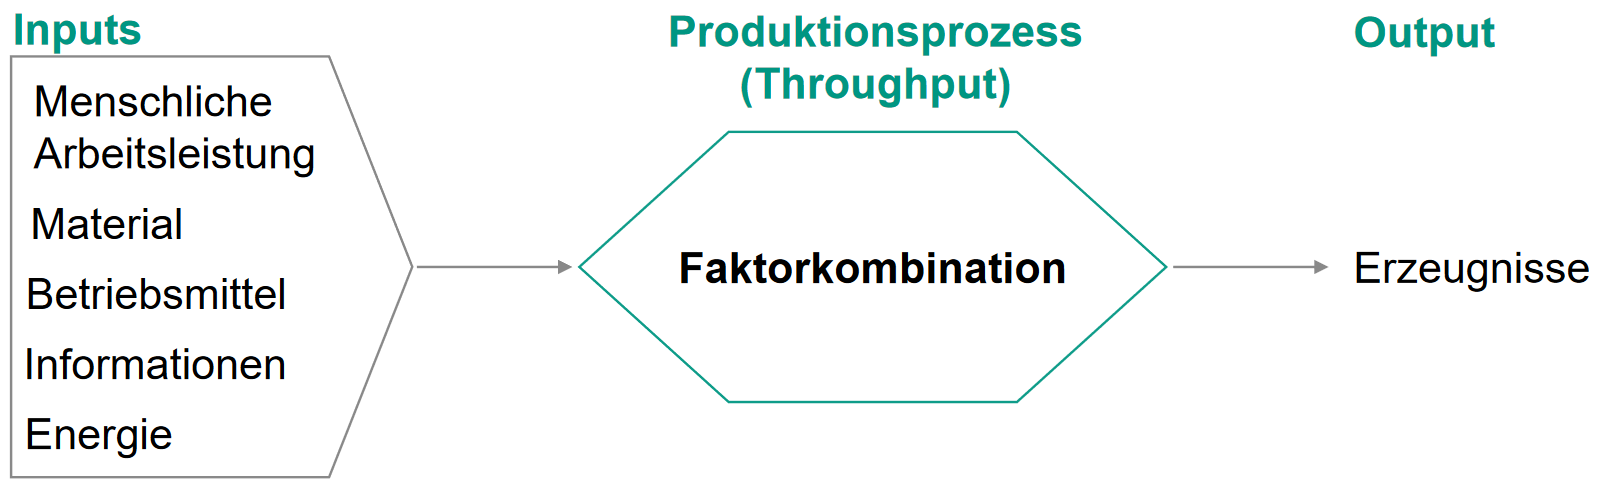
\includegraphics[width=0.7\textwidth]{images/prod-def.png}
\end{center}

\textbf{Produzierendes Gewerbe} (sekundärer Sektor, industrieller Sektor) umfasst:
\begin{itemize}
	\item Bergbau und Gewinnung von Steinen und Erden
	\item Verarbeitendes Gewerbe
	\item Energieversorgung und Wasserversorgung
	\item Baugewerbe
	\item ca. 25\% der Erwerbstätige und des BIPs in Deutschland
\end{itemize}
\bigskip
\textbf{Produktion im Unternehmenskreislauf:}
\begin{center}
	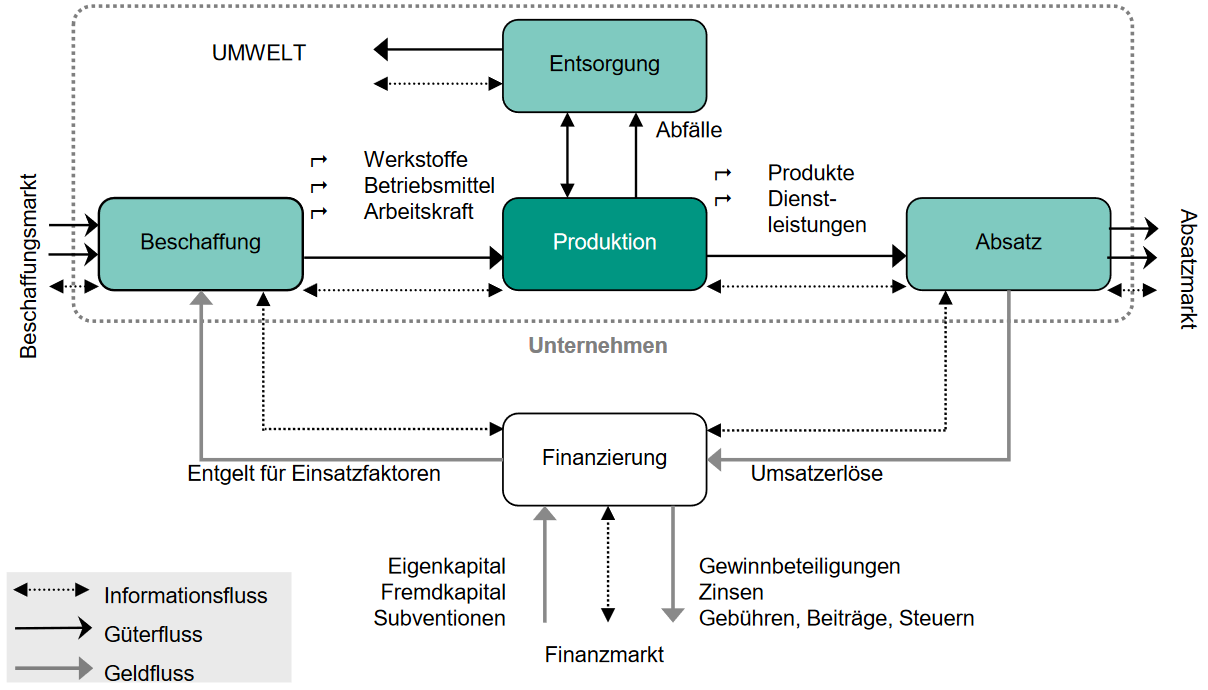
\includegraphics[width=0.8\textwidth]{images/production-circuit.png}
\end{center}
\begin{itemize}
	\item \textbf{Wertschöpfung}: Verkaufswert des Outputs minus Wert für extern bezogene Güter und Dienstleistungen
	\item \textbf{Wertschöpfungskette}: \textit{siehe Supply Chain Definition S.2}
\end{itemize}
\pagebreak
\textbf{Wichtige Teilgebiete der Produktion:}
\begin{itemize}
	\item \textbf{Produktionsplanung}: Systematische Identifikation, Bewertung und Auswahl von
	Handlungsmöglichkeiten $\rightarrow$ Optimale Erfüllung der strategischen Vorgaben
	\item \textbf{Produktionssteuerung}: Umsetzung der Produktionspläne im täglichen Produktionsablauf
	\item \textbf{Produktionsmanagement}: Konkretisierung und Umsetzung der strategischen Vorgaben der Unternehmensführung im Bereich der betrieblichen Leistungserstellung
\end{itemize}
\bigskip
\textbf{Planungsaufgaben des Produktionsmanagements} (\textit{s. S.3/4}):
\begin{itemize}
	\item \textbf{Strategisches Produktionsmanagement}: Strategien zur Schaffung und Erhaltung einer leistungsfähigen Produktion und Wettbewerbsfähigkeit
	\item \textbf{Taktisches Produktionsmanagement}: Konkretisierung der Strategien, Entscheidungen über Leistungsfelder und Technologien
	\item \textbf{Operatives Produktionsmanagement}: Optimaler Einsatz des vorhandenen Produktionsapparates, z.B. durch Produktionsprogrammplanung, Materialwirtschaft, Ablaufplanung
	\item \textit{Beispiele siehe Produktion VL 1, F21,23,25,26}
\end{itemize}
\bigskip
\textbf{Nachhaltige Produktion}:
\begin{itemize}
	\item \textbf{Definition Nachhaltigkeit}: Erfüllung der vorherrschenden Bedürfnisse ohne zukünftige Generationen daran zu hindern ihre Bedürfnisse zu erfüllen
	\item \textbf{Prinzipien}: Intergenerationale und intragenerationale Gerechtigkeit
	\item \textbf{Drei Säulen-Konzept der Nachhaltigkeit}: Ökonomische Sicherheit, Ökologisches Gleichgewicht, Soziale Gerechtigkeit
	\item \textbf{3 P der Nachhaltigkeit}: Prosperity (Profit), Planet, People
	\item PLE durch \textbf{Sustainable Development Goals} (\textit{VL1, F34}) und \textbf{European Green Deal} (\textit{VL1, F32}) in Richtung Nachhaltigkeit verändert
	\item \textbf{Nachhaltige Wertschöpfungsketten} (\textit{VL1, F37-48})
\end{itemize}
\pagebreak
\textbf{Von der Linearwirtschaft zur Kreislaufwirtschaft - Circular Economy:}
\begin{center}
	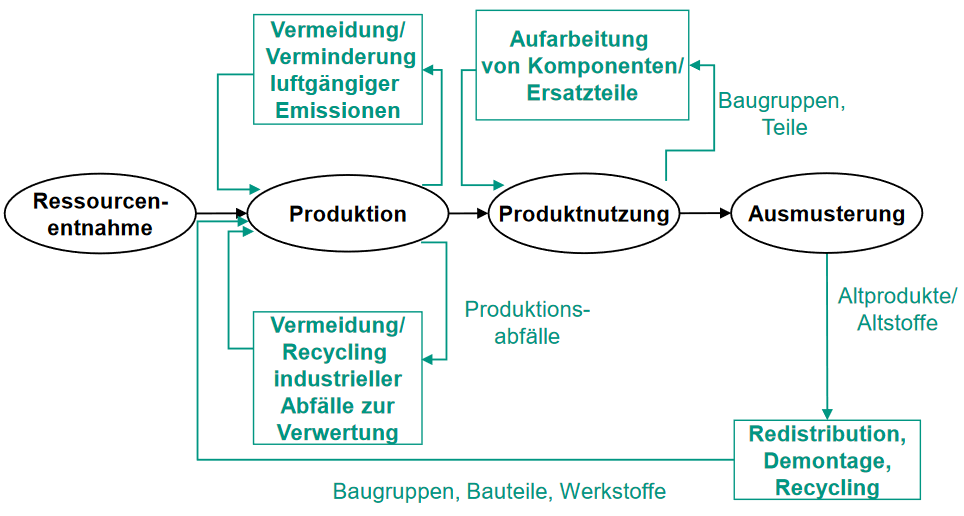
\includegraphics[width=0.7\textwidth]{images/circular-economy.png}
\end{center}




